The ``program counter circuit'' is the loop formed by the Program Counter along with the Branch and Jump circuitry, see figure \vref{figure:pc-circuit}.

The program counter is a register that holds the address of the next instruction to be fetched.
When no branching or jumping is involved (the ``sunny day scenario''), the program counter cycle updates the program counter when the control unit tells it to.
This means that the control unit is the entity that advances the running program.
The control unit advances the program counter when it is in the execute state, so that a new program counter value is ready for when the control unit enters the fetch state.

When the program counter is updated the Program Counter Out signal is set to equal the Program Counter In signal.

When the control unit gives the signal, a branch or jump is performed by manipulating the program counter circuit to change the value sent back to the program counter.

\begin{figure}[h!]
	\begin{center}
		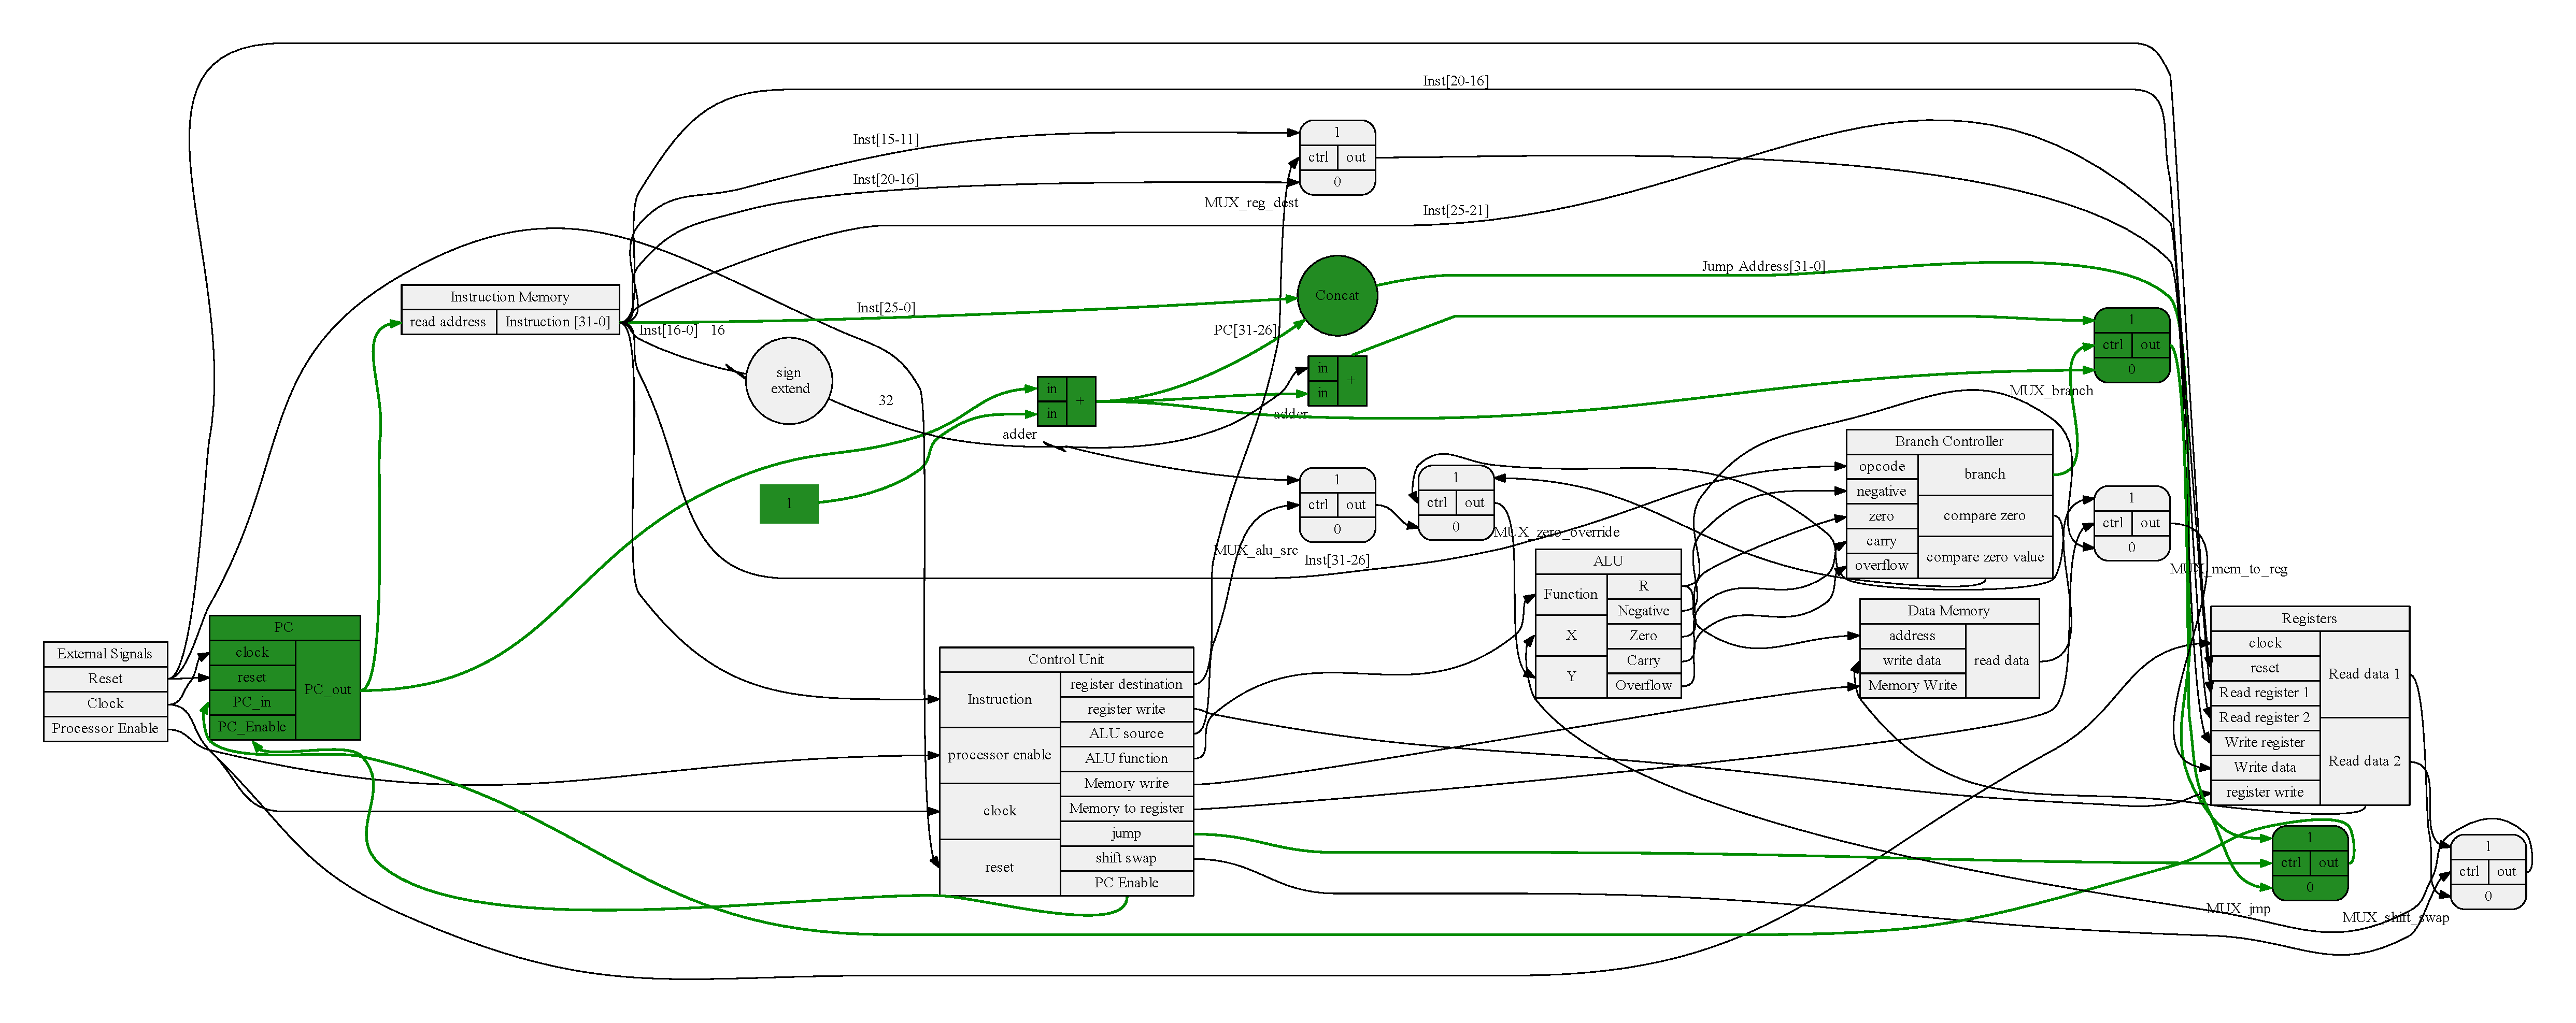
\includegraphics[keepaspectratio, height=\textheight, width=\textwidth]{graphics/cpu-architecture/cpu-arc-pc-circuit.pdf}
		\caption{Architecture of the solution processor. The signals and components directly involved with the program counter circuit are highlighted in green.}
		\label{figure:pc-circuit}
	\end{center}
\end{figure}


\subsubsection{Program Counter}

The program counter is implemented as a D-type flip-flop with reset and enable signals.

\subsubsubsection{In Signals}

\begin{description}
\item{\textbf{Clock}} \\

Clock signal.

\item{\textbf{Program Counter In}} \\

The Program Counter's next value.

\item{\textbf{Reset}} \\

When the reset signal is high, the program counter is reset to $-1$\footnote{\texttt{FF FF FF FF}} on the next rising edge of the clock.

\item{\textbf{Program Counter Enable}} \\

Tells the Program Counter whether or not the Program Counter should be updated.
When this signal is \texttt{1} the Program Counter is updated.

\end{description}

\subsubsubsection{Out Signals}

\begin{description}
\item{\textbf{Program Counter Out}} \\

The Program Counter Out signal is the address of the current instruction.

\end{description}

For more information about how the program counter circuit works, refer to figure \vref{figure:pc-circuit}.
